%%%%%%%%%%%%%%%%%%%%%%%%%%%%%%%%%%%%%%%%%%%%
% Chapitre 6
%%%%%%%%%%%%%%%%%%%%%%%%%%%%%%%%%%%%%%%%%%%%

\chapter{Caractérisation des changements}
\label{Chapter6}

Le \chapref{Chapter4} présente des méthodes de détection de changements entre deux populations de tenseurs.
Ces méthodes de comparaison de groupes permettent de détecter les régions pour lesquelles la forme des tenseurs de diffusion diffère 
significativement d'une population à l'autre, sans toutefois donner d'information sur la nature des changements observés.
Ainsi, une méthode complémentaire est proposée, permettant de caractériser a posteriori les changements détectés en termes de
modification de la Fraction d'Anisotropie (FA), Diffusion Moyenne (DM), Diffusion Radiale (DR) ou Diffusion
Axiale (DA), afin de rendre l'interprétation des résultats plus aisée pour le Neurologue.\\

% \minitoc

%----------------------------------------------------------------------------------------

\section{Post-traitement général}
Les cartes de \textit{p-valeurs} obtenues en sortie des méthodes de détection des changements sont dites \og brutes \fg,
c'est-à-dire sans avoir subies de transformations quelconques pour améliorer les détections.
Nous les appellerons par la suite \og cartes primaires \fg.
Il est possible d'appliquer, de manière systématique, des corrections statistiques et morphologiques à ces cartes.
Le post-traitement général présenté dans cette section est effectué en deux étapes : 
une correction statistique des cartes de \textit{p-valeurs} suivie d'une correction sur la topologie des détections.
Après ces corrections, la carte de résultats est appelée \og carte corrigée \fg.

\subsection{Correction statistique des cartes de p-valeurs}
Positionnons-nous dans le cas de la compraison de groupes en imagerie médicale.
Nous avons $N$ images-sujets comportant $V$ voxels chacune.
Le \mlg va réduire pour chaque voxel les $N$ informations en $K$ régresseurs et 
le test statistique va mesurer l'effet d'un de ces régresseurs pour chaque voxel.
En sortie, nous obtenons une carte de $V$ \textit{p-valeurs} (carte primaire de détection).
Durant ce processus, le test d'hypothèse \eqref{test_stat} est effectué $V$ fois.
Ces $V$ tests sont indépendants et pour chacun le niveau de signification est nommé $\alpha_{test}$. 
Il correspond à la probabilité de rejeter l'hypothèse nulle $\mathcal{H}_0$ alors qu'elle est vraie, 
ou encore à la probabilité de détecter un Faux Positif.
Sur ces $V$ tests, nous connaissons le nombre $A$ de décisions acceptant l'hypothèse $\mathcal{H}_0$ et le nombre $R$ la rejetant ($V=A+R$).
Trois cas sont possibles : \\
\begin{itemize}
    \item Sans aucune correction, un pourcentage $\alpha_{test}$ des $V$ voxels sont des Faux Positifs.\\
    
    \item Le premier type de correction sert à contrôler le nombre de Faux Positifs parmi le $V$ voxels.
    C'est la méthode de Bonferroni \cite{Abdi2007} (ou encore en anglais \textit{Family Wise Error Rate} FWER).
    Les $V$ tests sont indépendants donc la probabilité d'accepter l'hypothèse nulle $\mathcal{H}_0$ pour cette famille de test est : $(1-\alpha_{test})^V$.
    Il en découle directement la probabilité de rejeter $\mathcal{H}_0$ pour la famille de test : $\alpha_{famille} = 1 - (1-\alpha_{test})^V$.
    Par exemple, si $V=100$ et $\alpha_{test} =0.05$ alors $\alpha_{famille}=0,00592$.
    Pour une image classique du tenseur de diffusion avec une taille de $128\time128\time41$, nous avons $V=671744$ voxels.
    Alors la probabilité $\alpha_{famille}$ devient très petite, rendant la correction trop stricte.\\
    
    \item La deuxième méthode de correction va contrôler le nombre de Faux Positifs $FPos$ parmi les $R$ détections \cite{Benjamini1995, Benjamini2001}
    (en anglais \textit{False Discovery Rate} FDR).
    Il définit un taux de Faux Positif $taux_{FPos}$ et exprime le FDR comme l'espérance de ce taux devant être inférieur au niveau de signification $\alpha_{test}$ :
    \begin{align}
        taux_{FPos} &= \left\{ \begin{array}{lr} \frac{FPos}{R} & : R > 0\\ 0 & : sinon \end{array} \right.\\
        FDR &= E\left[taux_{FPos} \right] < \alpha_{test}
    \end{align}
    La procédure consiste à classer les $R$ \textit{p-valeurs} : $p_1 \leq p_2 \leq \dots p_R$ par ordre croissant.
    Et à rejeter les $k$ \textit{p-valeurs} (parmi les $R$) qui vérifient :
    \begin{equation}
        p_i \leq \frac{i}{V}\alpha_{test} 
    \end{equation}
    Avec cette correction, seuls $\alpha_{test}$ voxels sur les $R$ sont des fausses alarmes (Faux Positifs).
    Pour notre chaine de traitements, nous avons choisi cette correction.
\end{itemize}


\subsection{Composantes connexes}
La correction statistique permet de contrôler le taux de Faux Positifs sur l'image entière
mais ne fait aucune intervention par rapport à la morphologie des zones détectées.
Physiquement, il est facile de comprendre que les détections de voxels isolés ou encore des agrégats de voxels de toutes petites tailles, ne sont pas représentatifs d'une lésion 
car elles sont, de manière générale, plus étendues sur la substance blanche.
Par exemple, pour une image de résolution $1.8\time1.8\time3.5 mm^3$, une détection isolée (1 seule voxel) corresponderait à une lésion d'environ $12 mm^3$.
Ces détections sont souvent attribuées à de Faux Positifs.
Par la suite, il est préférable de ne conserver que les agrégats dont la taille est supérieure à celle fixée par l'utilisateur (voir \figref{etape_carac_1}).
Pour cela, nous utilisons la méthode des composantes connexes.
Ce sont des opérateurs de morphologie mathématique qui servent, généralement, d'outils de filtrage et de segmentation.

\begin{figure}[ht]
  \centering
  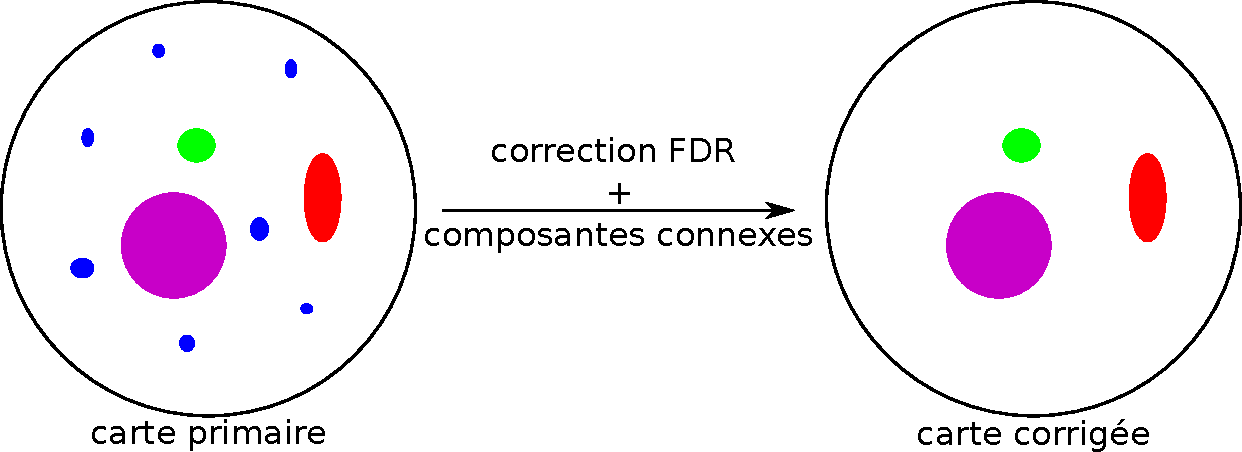
\includegraphics[scale=0.5]{Images/etape_carac_1.pdf}
  \caption{\label{etape_carac_1}Illustration du post-traitement général.}
\end{figure}


\section{Caractérisation des zones détectées}
Les méthode de comparaison de groupes basées sur les tenseurs sont des extension du \mlg.
Avec le test de Fisher introduit au \chapref{Chapter4}, une carte de \textit{p-valeurs} est obtenue.
Elle est ensuite corrigée par la méthode du False Discovery Rate (FDR), puis seuillée à un seuil de 5\%.
Cette approche permet d'identifier les régions atteintes par la pathologie, sans apporter d'information sur la nature et le sens des changements détectés.
Cette section présente une méthode de post-traitement pour pallier à la problématique des méthodes de détection.
Elle consiste à caractériser les détections obtenues avec les méthodes du \chapref{Chapter4}.


\subsection{Description de la méthode de caractérisation}
Les méthodes de comparaison de groupes permettent de prendre en compte toute l'information contenue dans les tenseurs sous différentes hypothèses
(homoscédasticité et hétéroscédasticité).
Pour chaque méthode, des régresseurs associé à chaque élément du tenseur, sont estimés au sens des moindres carrés.
Ensuite, un test statistique de Fisher est utilisé pour tester la significativité des effets de ces regresseurs dans les modèles.

La première étape (voir \figref{etape_carac_1}) de la caractérisation des changements consiste à corriger les cartes de détection par la méthode du FDR,
puis à étiqueter les composantes connexes de la carte des détections seuillée 
et à ne conserver que celles dont la taille est supérieure à un seuil fixé par l'utilisateur. 
Cette étape correspond aux opérations du post-traitement général.

\begin{figure}[ht]
    \centering
    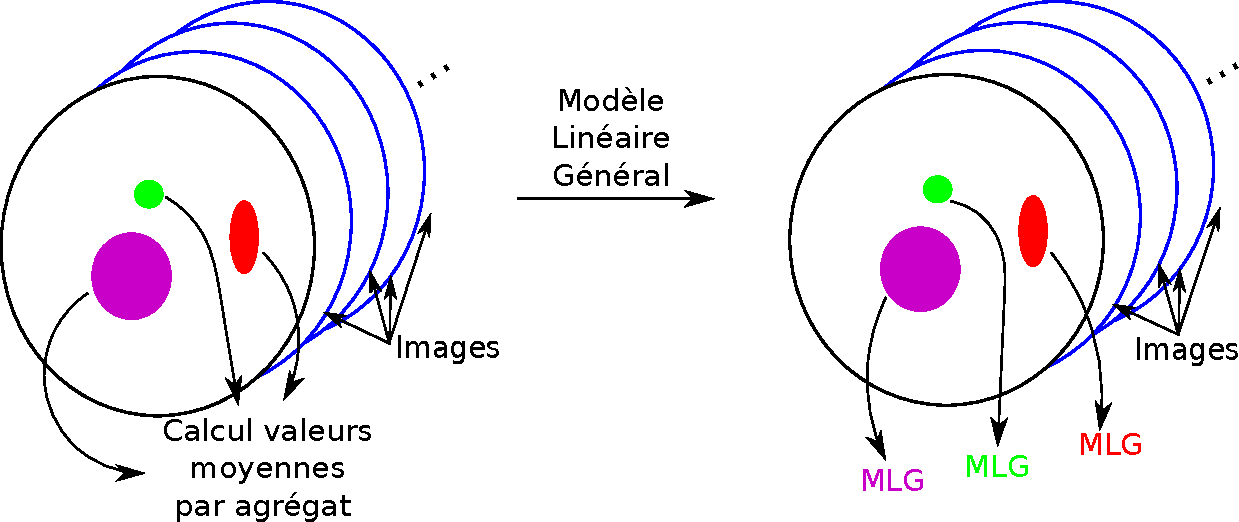
\includegraphics[scale=0.6]{Images/etape_carac_2.pdf}
    \caption{\label{etape_carac_2}Illustration de la deuxième étape de la caractérisation.}
\end{figure}
La deuxième étape (voir \figref{etape_carac_2}) consiste, sur chaque région et pour chaque sujet, à calculer les valeurs
moyennes des différents indices scalaires (\fa (FA), \md (DM), \dr (DR) et \da (DA)) et à comparer indépendemment chacune de ces quantités grâce à
un \mlg, en utilisant les même covariables que précédemment.

\begin{figure}[ht]
    \centering
    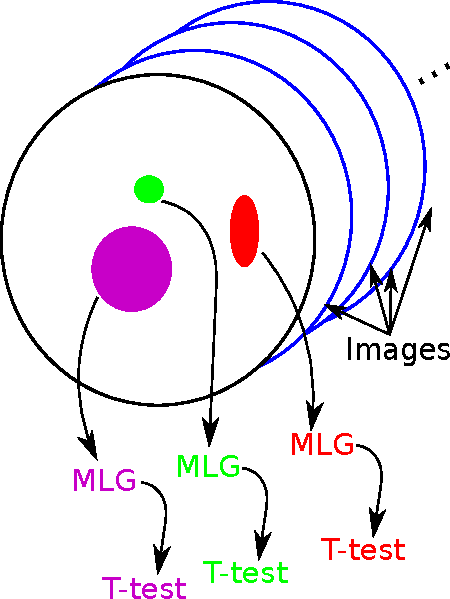
\includegraphics[scale=0.6]{Images/etape_carac_3.pdf}
    \caption{\label{etape_carac_3}Illustration de la troisième étape de la caractérisation.}
\end{figure}
Un test de Student, ou encore T-test, est réalisé pour chaque agrégat, afin d'identifier le sens du changement détecté (voir \figref{etape_carac_3}).
L'hypothèse nulle $\mathcal{H}_0$ vérifie $c^t \hat{B} =0 \text{ avec } c \in \mathbb{R}^{k}$ 
le vecteur de constraste permettant de faire une combinaison linéaire des régresseurs $\hat{B}$.
\begin{equation}
    t = \frac{c^t\hat{B}}{\sqrt{c^t\hat{\Sigma}c}} \sim T_{d=N-K}
\end{equation}
Contrairement au test statistique utilisé \eqref{test_stat} pour les méthodes de détection,
il est alors possible de tester l'équalité entre deux régresseurs en mettant à $1$ et $-1$ les contrastes associés aux deux régresseurs à l'étude et tous les autres contrastes à $0$.
Ou encore, nous pouvons tester si un régresseur n'a pas d'effet sur le modèle en mettant le constraste associé à $1$ et les autres à $0$ pour, par exemple, étudier la corrélation supposée entre un score clinique et les observations.

Il faut noter une différence par rapport au cadre statistique précédent.
Dans le cas de ce test, pour la comparaison de groupes, il faut deux variables explicatives pour les deux groupe $\{x_1, x_2\}$ 
afin d'estimer un régresseur représentant le premier groupe et un deuxième pour l'autre groupe.


\subsection{Format de présentation des résultats}
La liste de ces régions est présentée au médecin en respectant l'ordre suivant dans les indices scalaire : DA:\da, DR:\dr, DM:\md, FA:\fa.
Seules les régions ayant conduit à au moins un test significatif au seuil de 5\% sont conservées. 
Cette liste précise le sens de modification du test à l'aide de deux symboles : ($+$) pour une augmentation et ($-$) pour une diminution, 
ainsi que le niveau de signification : ($n.s.$) pour un résultats non significatif.
Un exemple fictif, correspondant au schéma de la \figref{etape_carac_3}, est donné par le \tabref{ex_caracterisation}.
Les trois agrégats violet, vert et rouge correspondent respectivement aux numéros {\color{purple}1}, {\color{green}2} et {\color{red}3}.

\begin{table}[ht]
\centering
\begin{tabular}{|D{2cm}|D{1cm}|D{1cm}|D{1cm}|D{1cm}|}
      \hline
      \textbf{Agrégats} & \textbf{DA} & \textbf{DR} & \textbf{DM }& \textbf{FA} \tabularnewline
      \hline
      {\color{purple}1} & $-$ & $n.s.$ & $-$ & $-$\tabularnewline
      {\color{green}2} & $n.s.$ & $+$ & $+$ & $-$\tabularnewline
      {\color{red}3} & $-$ & $-$ & $-$ & $n.s.$\tabularnewline
      \hline
  \end{tabular}
  \caption{\label{ex_caracterisation}Exemple de liste présentant les résultats de la caractérisation.}
\end{table}

Dans la littérature \cite{Harsan2006}, deux types de modification ont été reliés à des phénomènes biologiques provoqués 
par des pathologies dégénératives du système nerveux central chez l'homme :\\
\begin{itemize}
    \item une diminution de la \da peut représenter une modification axonale comme une réduction du diamètre de l'axone.
    Cela engendrera aussi une diminution de la \md et de la Fraction d'Anisotropie.
    Dans ce cas de figure, les changements détectés en \dr ne sont pas représentatifs de la modification et nous admettons qu'ils peuvent être $-/+/n.s.$.
    La combinaison des symboles est : \{$-$, $(-/+/n.s.)$, $-$, $-$\}\\
    \item une augmentation de la \dr peut représenter une dégradation de la couche de myéline.
    Nous parlons alors de démyélinisation.
    Cela entraine une augmentation de la \md et une diminution de la Fraction d'Anisotropie.
    Dans ce cas là, les modifications détectées pour l'indice scalaire \da ne correspondent pas à des cas réels et les trois symboles $-/+/n.s.$ peuvent leur être attribués.
    La combinaison des symboles est : \{$(-/+/n.s.)$, $+$, $+$, $-$\}\\
\end{itemize}

Certaines combinaisons de symboles, par exemple \{$-$, $-$, $-$, $n.s.$\} ou encore \{$-$, $-$, $-$, $+$\}, 
représentent des modifications qui ne peuvent être associées avec des cas réels.
Deux explications permettent de comprendre ces résultats.
Tout d'abord, les changements détectés correspondent à une modification de l'orientation de la diffusion ce qui est impossible à détecter avec les valeurs scalaires.
Ensuite, il est possibile que plusieurs modifications différentes soient présentes dans l'agrégat et en faisant la moyenne des valeurs scalaires, 
les différents changements se compensent les uns aux autres.


\begin{figure}[ht]
    \centering
    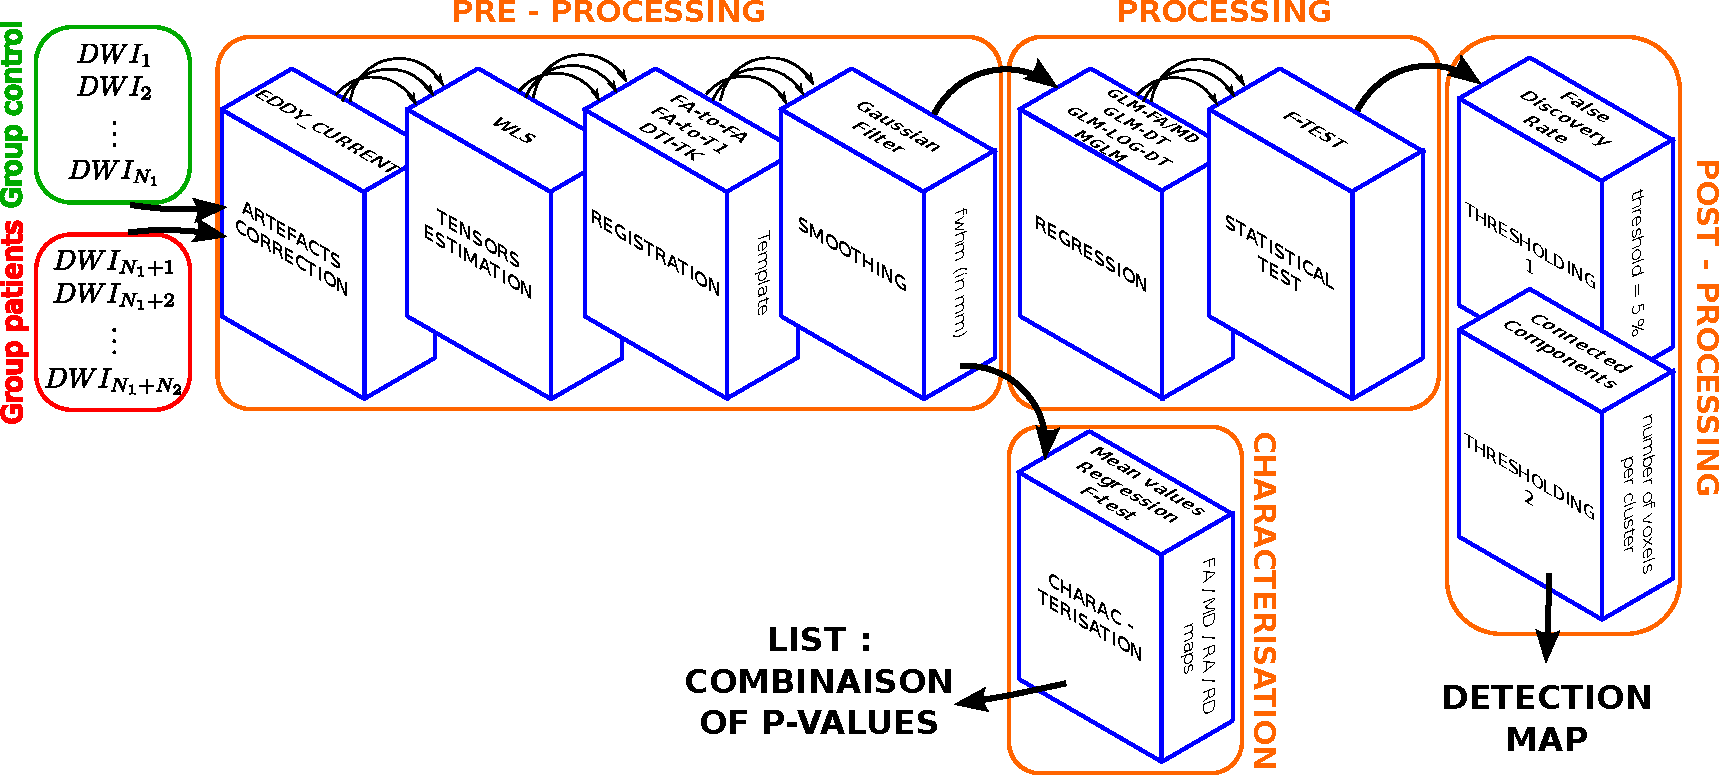
\includegraphics[width=1\textwidth]{Images/pipeline.pdf}
\end{figure}
